\begin{frame}
\frametitle{Solution to the batched Approach}
\begin{Large}
How can we improve the batched approach? 
\end{Large}
\begin{itemize}
\item A batch without double appearing words? 
\item Analyze the distribution of words in the dataset?
\item Creating the perfect batch? 
\item Delete frequent occuring words from the dataset? 
\end{itemize}
  \end{frame}
  \begin{frame}
\frametitle{Distribution of Words}
\begin{Large}
Problem:\\
\end{Large}
Words appear more than once in a batch $\rightarrow$ performance loss\\
\begin{Large}
Solution:\\
\end{Large}
Create batch of different sizes, each batch will hold at most one pair per context word\\
\begin{large}
Problem of the Solution:\\
\end{large}
Average Batch Size = 200, i.e training takes too long
  \end{frame}
\begin{frame}
\frametitle{Distribution of Words}
\centering
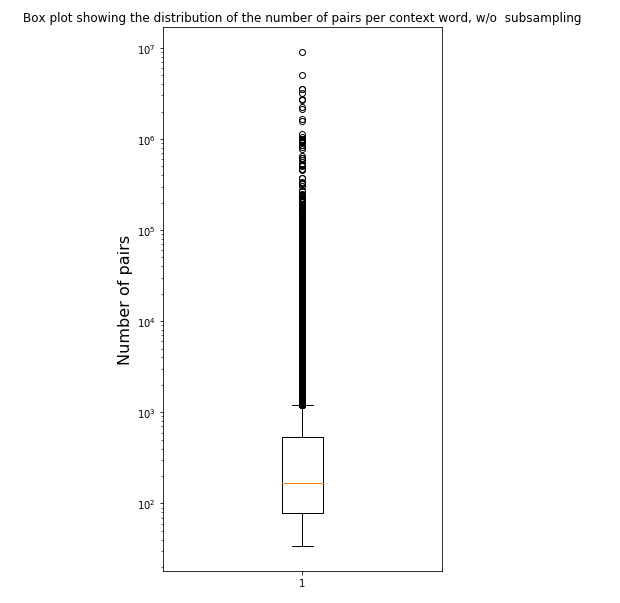
\includegraphics[scale=0.2]{images/no_sampling_boxplot}
  \end{frame}
\begin{frame}
\frametitle{Distribution of Words}
\begin{Large}
Results of the Distribution
\end{Large}
\begin{itemize}
\item A few words are responsible for the majority of pairs. 
\item They almost have the same context words
\item Have they the same representation? 
\end{itemize}
  \end{frame}
  \begin{frame}
\frametitle{Distribution of Words}
\begin{Large}
Yes they have!
\end{Large}
blablalbab
  \end{frame}
    \begin{frame}
\frametitle{Deletion of outliers}
\begin{Large}
First Results 
\end{Large}
  \end{frame}
      \begin{frame}
\frametitle{Deletion of outliers}
\begin{Large}
Future Work 
\end{Large}
\begin{itemize}
\item Creating the perfect batch 
\item Analyze the deletion of outliers on other (bigger) datasets.
\end{itemize}
  \end{frame}